\documentclass{article}

\usepackage[margin=0.5in]{geometry}
\usepackage{graphicx}
\usepackage{subcaption}

\begin{document}

\title{Rotating Flow in Cavity: Rarefaction Effects}
\author{Lambert Theisen}
\maketitle

\begin{itemize}
  \item Geometry and BCs form Fig.~\ref{fig:geometry}.
  \item In Fig.~\ref{fig:paradox}, we observe increasing maximum velocity with increasing Knudsen number, reaching a plateau and then decreasing for higher Knudsen numbers.
  \item In Fig.~\ref{fig:velocity_fields}, we see that the direction of the vortex flips at some point.
\end{itemize}

\begin{figure}[ht]
  \centering
  \begin{subfigure}{0.35\textwidth}
    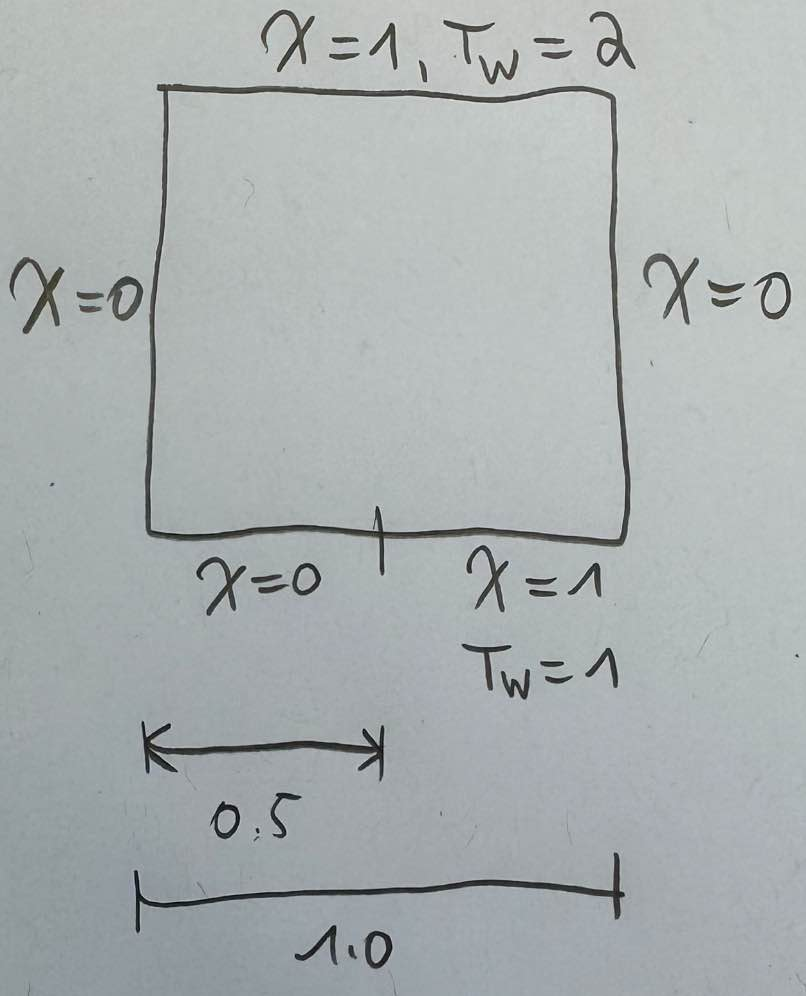
\includegraphics[width=\textwidth]{sketch.jpg}
    \caption{Geometry and Boundary Conditions}\label{fig:geometry}
  \end{subfigure}
  \begin{subfigure}{0.6\textwidth}
    \includegraphics[width=\textwidth]{fig.pdf}
    \caption{Maximum velocity \(\max \|\textbf{u}\|_2\) vs Knudsen number \(\textnormal{Kn}\)}\label{fig:paradox}
  \end{subfigure}
\end{figure}

\begin{figure}[ht]
  \centering
  \begin{subfigure}{0.36\textwidth}
    \includegraphics[width=\textwidth]{results_rotating_cavity0.010737418240000001/u_0.pdf}
    \caption{\(\textnormal{Kn} = 0.0107\)}
  \end{subfigure}
  \hspace{-1.0cm}
  \begin{subfigure}{0.36\textwidth}
    \includegraphics[width=\textwidth]{results_rotating_cavity0.02097152/u_0.pdf}
    \caption{\(\textnormal{Kn} = 0.0209\)}
  \end{subfigure}
  \hspace{-1.0cm}
  \begin{subfigure}{0.36\textwidth}
    \includegraphics[width=\textwidth]{results_rotating_cavity0.04096/u_0.pdf}
    \caption{Velocity Contour Plot}
  \end{subfigure}
  \begin{subfigure}{0.36\textwidth}
    \includegraphics[width=\textwidth]{results_rotating_cavity0.08000000000000002/u_0.pdf}
    \caption{\(\textnormal{Kn} = 0.0800\)}
  \end{subfigure}
  \hspace{-1.0cm}
  \begin{subfigure}{0.36\textwidth}
    \includegraphics[width=\textwidth]{results_rotating_cavity0.15625/u_0.pdf}
    \caption{\(\textnormal{Kn} = 0.1563\)}
  \end{subfigure}
  \hspace{-1.0cm}
  \begin{subfigure}{0.36\textwidth}
    \includegraphics[width=\textwidth]{results_rotating_cavity0.30517578125/u_0.pdf}
    \caption{\(\textnormal{Kn} = 0.3052\)}
  \end{subfigure}
  \begin{subfigure}{0.36\textwidth}
    \includegraphics[width=\textwidth]{results_rotating_cavity0.5960464477539062/u_0.pdf}
    \caption{\(\textnormal{Kn} = 0.5960\)}
  \end{subfigure}
  \hspace{-1.0cm}
  \begin{subfigure}{0.36\textwidth}
    \includegraphics[width=\textwidth]{results_rotating_cavity1.8189894035458565/u_0.pdf}
    \caption{\(\textnormal{Kn} = 1.8190\)}
  \end{subfigure}
  \hspace{-1.0cm}
  \begin{subfigure}{0.36\textwidth}
    \includegraphics[width=\textwidth]{results_rotating_cavity4.440892098500626/u_0.pdf}
    \caption{\(\textnormal{Kn} = 4.4409\)}
  \end{subfigure}
  \caption{Velocity field}\label{fig:velocity_fields}
\end{figure}
\end{document}
